\chapter{Conception and Realisation}
\label{chapter:conception}

\section{Literature and basics :}
At the beginning, it was necessary to acquire some basics about quantum mechanics (density matrix, Maxwell-Bloch equations..) by reading some introductory literature ~\cite{bastard1992}. A concrete example for the simulation and the numerical solving of the Maxwell-Bloch system was described in the paper of Ziolowski.\\
QuTiP, a Python Toolbox for simulating the dynamics of open quantum systems, was the starting point with . It offered a variety of examples in the field of Quantum mechanics using Jupyter Notebooks: they are designed to expose code blocks with human-friendly text which makes data analysis easier to share and reproduce, an interactive tool to describe quantum mechanic systems.\\
\section{Python/C++ Interface :}
After handling some basics, I started searching for the possibilities to create the Python/C++ Interface:\\
\begin{itemize}
\item Python Boost : Boost.Python is an open source C++ library which provides an interface for binding C++ classes and functions to Python. It does enable a safe wrapping C++ functions that return by reference, with call policies, which force the user to define how to handle the reference counts of raw pointers and reference returns at wrapper-compilation time. It also allows what are effectively templated typemaps (create automatic conversions for templated array or matrix classes that don't require any boilerplate or declarations of what template instantiations will be used). But Boost.Python uses extensively C++ template. They can lead to compilation problems. Moreover, templates use a huge amount of memory. \\
\item ctpyes : ctypes is a convenient way to reach for a few functions within a DLL when the calls happen outside of a key bottleneck, not as a way to make large C libraries available to Python in performance-critical situations.\\
\item SWIG (Simplified Wrapper and Interface Generator): It is a language neutral compiler that turns ANSI C/C++ declarations into scripting language interfaces.It targets Python, Tcl, Perl, MATLAB, etc..
one of the its important features is that it is simple and completely automated (generates a fully working Python extension module).
Although it doesn't have the efficiency of Python Boost regarding  templated typemaps, it does have tha advantage of supporting general typemaps for C++ lvalues (non-const references or pointers) and changing the conversion and matching behavior for built-in C++ and Python types. Keeps both the C++ and Python code clean, i.e. not altering Python itself.\\
\end{itemize}
So I installed SWIG and learned how to create a Python module starting from an interface file and a header file. The next step was to wrap a C++ class in order to create instances of this class and modify its attributes in the Python Testprogram. (see Fig. \ref{fig:swig})\\
\begin{figure}[htb]
  \centering
  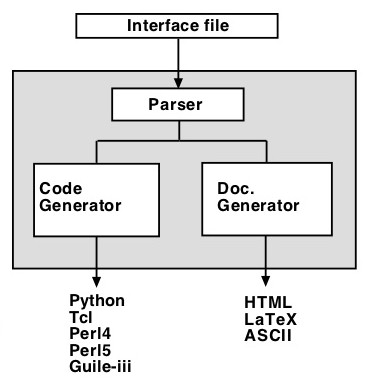
\includegraphics[width=0.5\textwidth]{figures/swig}
  \caption{SWIG}
  \label{fig:swig}
\end{figure}
\section{Serialisation of Metadata :}
The next point to handle was the Metadata, how to extract them from an XML File and then store them with results at the end. Here i used dexml which is a simple object-XML mapper for Python, to serialize the Metadata and save it as Python Objects.\\
\section{Storing results :}
Furthermore i looked for the possible File format for the simulation results, that lead to the following options:\\
*XML : XML's biggest advantage is that it provides developers with a tool that concisely and unambiguously defines the format of data records. However it is not suitable for large amount of data.\\
*VTK : It is a powerful tool to viisualize scalars, vectors, complex numbers.. but  requires a diffcult setup and an understanding of the framework.\\
*CDF : \\
*HDF5 : HDF5 is a data model, library, and file format for storing and managing data. It supports an unlimited variety of datatypes, and is designed for flexible and efficient I/O and for high volume and complex data. HDF5 is portable and is extensible, allowing applications to evolve in their use of HDF5. The HDF5 Technology suite includes tools and applications for managing, manipulating, viewing, and analyzing data in the HDF5 format. \\ 
\section{Git :}
After settling the C++ library that contains all the necessary classes and functions and using SWIG to incorporate it in Python, choosing dexml for serialisation of metadata and HDF5 for storage of results, I acquired some knowledge about Git and created my own project that gathered all the pieces together. It is a mighty tool that allows users to coordinate work on projects between each other.\\\section{Makefile/CMake :}
To get more experience in handling scientific projects, I dedicated some time to understand the process of Makefiles and then CMake and applied them on my work. Makefiles are a simple way to organize code compilation, through rules specfied as as a list of target entries, in order to build executable programs from many modules. It only rebuilds in case of new modules added to the program. Furthermore, CMake is a cross platform build system, that automatically generates Makefiles for different platforms.
